\label{chap:arch}

\begin{figure*}[ht] \centering
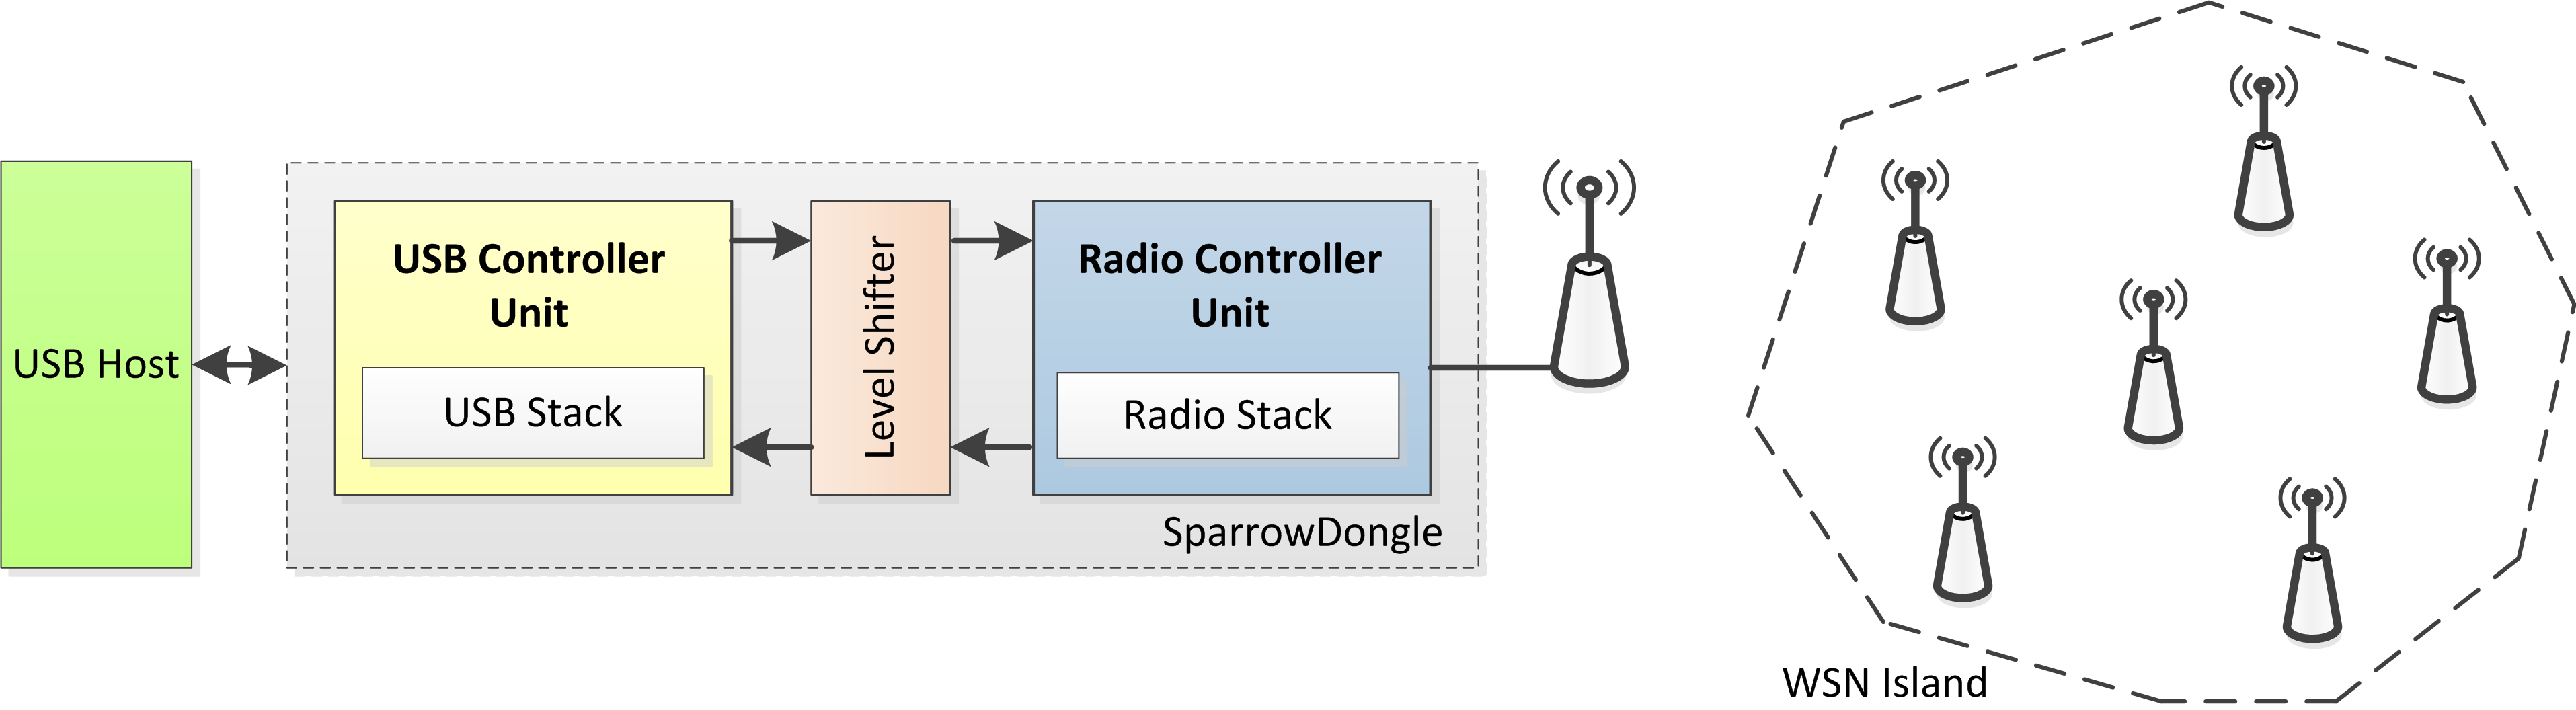
\includegraphics[width=0.9\textwidth]{img/Architecture.png}
\caption{SparrowDongle stick architecture} \end{figure*}

The canonical implementation for Atmel Zigbee transceivers is a USB stick
device with a USB controller and radio transceiver, which means that the USB
controller unit (the only controller present) on the device is responsible for
both radio and USB stack communication.  This lack of separation between key
functions of the gateway platform leads to the undesirable effect of software
for the USB stack competing for MCU time with the wireless stack. This greatly
limits both the USB throughput, features of the device and the complexity of
the wireless stack. The wireless stack in this scenario cannot have tight
timings built around receiving and transmitting packets on the wireless link,
as transfer to and from the microcontroller unit (MCU) is both slow and delayed
by (possible) USB tasks running asynchronously.

Our implementation differs in that respect by including two separate
controllers on the gateway device, one for USB communication and the other for
the 2.4Ghz Zigbee stack. This approach has several key advantages, described in
sections \ref{sec:func} and \ref{sec:homo}. 

Additionally, a number of design features were included for ease-of-use in
research and development, outlined in \ref{sec:pro}, \ref{sec:ant}


\subsection{\textit{Separation of functionality}} 

\label{sec:func}

USB communication is poll-based and initiated by the USB host. The
SparrowDongle stick acts as a USB device and its role requires frequent (every
millisecond) and low-latency communication with the USB host. Having two
controllers, the RF controller can run any RF communication stack
without having the USB code intrude on key timings. The serial link that
connects the two controllers has both sufficient speed and simplicity to allow
each controller to dedicate most computing cycles to handling communication on
the USB and wireless links, respectively.

\subsection{\textit{Homogeneity}}  

\label{sec:homo}

The components used for the RF communication in the SparrowDongle stick are
identical to those used for the Sparrowv3.2 nodes, thus they can share the same
codebase (As opposed to having an implementation for 8-bit AVR and an
implementation for ARM/x86). In many cases, gateways run on different
architectures than wireless sensor nodes and require stacks re-purposed for
that specific architecture (or for that platform, in the case of the canonical
Atmel implementation of the gateway). SparrowDongle eliminates the need for a
different branch of the same wireless stack since the code running on the
gateway is virtually identical to that running on any sensor node.

\subsection{\textit{Ease of programming}} 

\label{sec:pro}

SparrowDongle offers an easy-to-use programming and debugging interface for
both the USB controller and the RF controller. To keep the overall size of the
device small, we used shared ISP (In-System-Programming) and JTAG (Joint Test
Action Group) headers for programming the two controllers. This only requires
an ISP header, a JTAG header and two headers for jumper selection (One jumper
connects the ISP signal SCK to the respective SCK signal pin on one of the
controllers, the other connects the JTAG signal TCK to its respective signal
pins on one of the controllers), as shown in Figure \ref{fig:progr}.


\begin{figure}[ht] \centering \label{fig:progr}
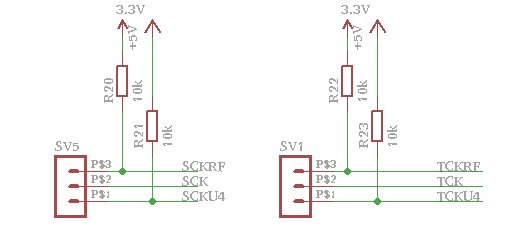
\includegraphics[width=0.35\textwidth]{img/progr.png} \caption{Header selection
for programming clock signals} \end{figure}


\subsection{\textit{External Antenna}}

\label{sec:ant}

The design for the SparrowDongle wireless stick includes an optional UFL
connector for an external antenna, which greatly increases range. A large, 8dBi
omni-directional antenna mounted on both gateways and nodes would amount to
around 200 metres of communication range, well over the 70m measured with the
default antennas.



